\section{Segnali utilizzati}
Gli stati utilizzati dalla componente, e la loro funzione, sono elencati di seguito:
\\
\begin{lstlisting}
signal state_curr, state_future, state_last: state;
signal length, word_to_process, word_to_save: std_logic_vector (7 downto 0);
signal writing_counter  : INTEGER range 0 to 16385 := 0;
signal reading_counter    : INTEGER range 0 to 16385 := 0;
signal local_counter     : INTEGER range 0 to 8 := 0;
signal write_index       : INTEGER range 0 to 16 := 0;
constant READ_BOTTOM     : std_logic_vector (15 downto 0) := "0000000000000000";
constant WRITE_BOTTOM    : std_logic_vector (15 downto 0) := "0000001111101000";
\end{lstlisting}
I segnali \codeword{state_curr}, \codeword{state_future} e \codeword{state_last}, di tipo state, sono, come appare evidente, necessari al salvataggio dello stato corrente, futuro e passato. Lo stato corrente tiene traccia dello stato in cui si trova la FSM, ed esegue le istruzioni in esso contenute; lo stato \codeword{state_last}, invece, tiene traccia dell’ultimo stato visitato, al fine di capire la provenienza del flusso del componente, ed indirizzare correttamente ad un nuovo stato. \codeword{state_future}, infine, è necessario in quanto tra la convoluzione di un bit e l’altro, la macchina passa attraverso lo stato \textbf{S\_CONV}, è pertanto necessario tenere traccia dello stato a cui la macchina dovrà essere indirizzata dopo la visita dello stato \textbf{S\_CONV}.
\\\\
I segnali length, \codeword{word_to_process} e \codeword{word_to_save}, tutti di tipo \codeword{std_logic_vector (7 downto 0)} sono necessari per tenere traccia rispettivamente del numero di parole da leggere ed elaborare, della parola letta e da sottoporre al convolutore, e della parola elaborata e da salvare nella RAM.
\\\\
I segnali \codeword{writing_counter}, \codeword{reading_counter},  \codeword{local_counter} e \codeword{write_index} sono tutti indici e contatori necessari per indicizzare, nell’ordine, gli indirizzi di memoria su cui salvare, da cui leggere, e il numero di convoluzioni da effettuare, e i bit della parola da salvare su cui scrivere. \codeword{writing_counter} e \codeword{reading_counter} vengono sommati rispettivamente alle costanti \codeword{READ_BOTTOM} e \codeword{WRITE_BOTTOM}, ossia i valori delle porzioni iniziali e finali di memoria che indicano la parte di scrittura e lettura.

\section{Descrizione della FSM}
Viene mostrato in figura uno schema della FSM progettata:
\\
\begin{figure}[ht]
    \centering
    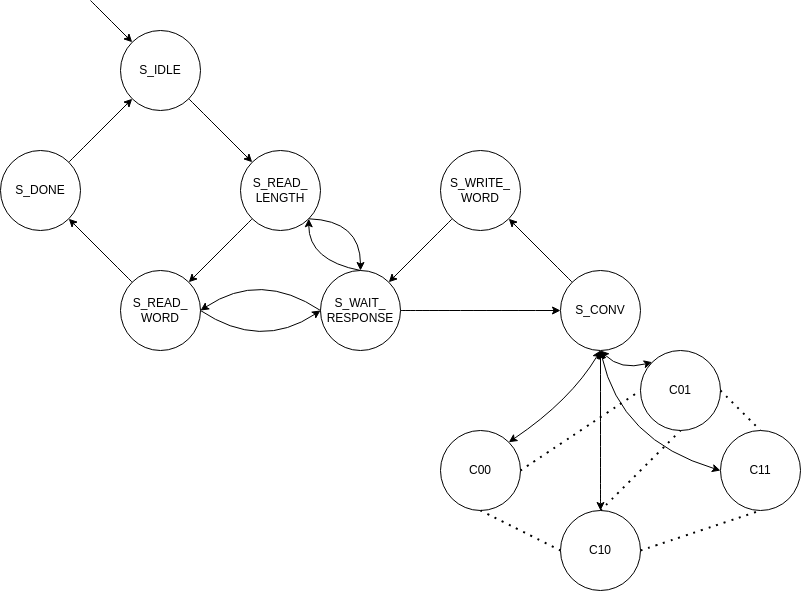
\includegraphics[width=\textwidth,height=0.74\textheight,keepaspectratio]{images/FSM.png}
    \label{fig:FSM}
\end{figure}
\\
Di seguito riportiamo gli stati utilizzati per progettare il comportamento del componente, associando ad ogni stato della FSM una specifica funzione spiegata qui sotto:
\begin{itemize}
    \item \textbf{S\_IDLE}: corrisponde allo stato di reset; vi si accede quando la componente riceve il segnale \codeword{i_rst}, serve all’inizializzazione dei valori necessari al funzionamento della macchina. Lo stato di reset persiste ad ogni giro di clock, fintanto che la componente non riceve un segnale di \codeword{i_start}.
    
    \item \textbf{S\_DONE}: corrisponde allo stato di fine elaborazione; è raggiungibile solo dallo stato \textbf{S\_READ\_WORD}, e vi si accede quando la sequenza di parole attese da elaborare è uguale al numero di parole in input elaborate. Lo stato \textbf{S\_DONE} porta alto il segnale \codeword{o_done} e abbassa invece lo stato \codeword{i_start}, raggiungendo, al successivo segnale di clock, lo stato \textbf{S\_IDLE}.
    
    \item \textbf{S\_READ\_LENGTH}: è lo stato deputato alla richiesta di lettura della lunghezza, ossia lo stato che richiede alla RAM la lettura (\codeword{o_en} = 1) della parola di memoria all’indirizzo 0000. Successivamente, reindirizza allo stato \textbf{S\_WAIT\_RESPONSE}, in attesa di risposta dalla RAM, e, al ritorno dal suddetto segnale, salva la lunghezza della sequenza attesa nello \codeword{std_logic_vector(7 downto 0)} ”length", successivamente reindirizza allo stato \textbf{S\_READ\_WORD}.
    
    \item \textbf{S\_READ\_WORD}: è lo stato deputato alla richiesta di lettura di una parola di memoria, il cui indirizzo è gestito dallo \codeword{std_logic_vector(7 downto 0)} \\ ”\codeword{reading_counter}", che viene incrementato ad ogni iterazione. Lo stato \\ \textbf{S\_READ\_WORD} si occupa inoltre di controllare se il numero di parole elaborate è minore della lunghezza di valori attesa; se così fosse, lo stato reindirizzerà allo stato \textbf{S\_WAIT\_RESPONSE}, per finalizzare la lettura (\codeword{o_en} = 1) e quindi per procedere con l'elaborazione della nuova parola; alternativamente, si verrà reindirizzati ad \textbf{S\_DONE}.
    
    \item \textbf{S\_WAIT\_RESPONSE}: è uno “stato cuscinetto”, utile in attesa della risposta della RAM, che, in quanto memoria asincrona, richiede un giro di clock per fornire alla componente interrogante una risposta di lettura e/o scrittura.
    
    \item \textbf{S\_WRITE\_WORD}: è lo stato deputato alla scrittura in memoria della parola elaborata. Vi si accede sempre e solo dallo stato \textbf{S\_CONV}, a seguito di 4 o 8 letture di bit in ingresso, ossia quando in output è pronta per il salvataggio una parola di 8 bit. Lo stato alza quindi i segnali di \codeword{o_en} e \codeword{o_we}, e provvede a scrivere all’indirizzo la cui gestione è affidata al segnale \codeword{writing_counter}, che viene incrementato ad ogni salvataggio. Successivamente si viene indirizzati allo stato \textbf{S\_WAIT\_RESPONSE}, al fine di permettere il salvataggio in memoria, e successivamente allo stato \textbf{S\_CONV} per continuare la convoluzione, o alla lettura di una nuova parola (stato \textbf{S\_READ\_WORD}), nel caso in cui siano stati consumati tutti i bit della parola in ingresso.
    
    \item \textbf{S\_CONV}: funge da controller della convoluzione, permette infatti di controllare, tra l’analisi di un bit e l’altra, se sono state eseguite 4 o 8 convoluzioni, ossia se sono state prodotte in output dal convolutore una o due parole, e se quindi è necessario andare a leggere un’ulteriore parola dalla memoria. Lo stato successivo a \textbf{S\_CONV} è, nel caso in cui siano state eseguite 4 o 8 convoluzioni, lo stato di scrittura in memoria della parola, mentre in tutti gli altri casi lo stato corrente viene indirizzato al \codeword{future_state} di cui si è tenuta traccia nell’ultima convoluzione di bit. Se il convolutore non ha mai ricevuto bit in ingresso, \codeword{future_state} sarà settato a C00.
    
    \item \textbf{C00, C01, C10, C11}: sono gli stati deputati alla convoluzione. Il loro funzionamento è descritto nel dettaglio nella sezione 1.3. Il segnale \codeword{future_state} tiene traccia del futuro stato di convoluzione da visitare, affinché vi ci si possa spostare una volta visitato lo stato \textbf{S\_CONV}, cosa che accade successivamente alla visita di ogni stato di convoluzione.
    
\end{itemize}